\section{Function Component} \label{sc:function_component}
Having added new attributes, classes, and structures to the class diagram through the model component, the functions from the function list can be implemented as well. Some of the functions should be implemented in the classes directly, others should be placed in the function component. The following section contains additions to the original function list, the arguments for these additions, decisions about implementations of these, and the final function component design.

\subsection{Additions to the function list}
The function list (see \autoref{tab:functions} on page \pageref{tab:functions}) has been constructed based on the original class diagram (see \autoref{fig:FirstPDClassDiagram}), but does not accommodate the new additions from the model component. To support the new classes, the following functions have been added:

\begin{table}[H]
\centering
    \begin{tabular}{c|l|l|l}
        \textbf{Nr.} & \textbf{Function name} & \textbf{Complexity} & \textbf{Function type}\\
        \hline
        1 & Get asset by id & Simple & Read\\
        \hline
        2 & Get department by id & Simple & Read\\
        \hline
        3 & Get tag by id & Simple & Read\\
        \hline
        4 & Search for tag & Medium & Compute/Read\\
        \hline
        5 & Add field to asset/tag & Medium & Update\\
        \hline
        6 & Update tag information & Complex & Update\\
        \hline
        7 & Update department information & Complex & Update\\
        \hline
    \end{tabular}
\end{table}

Functions 1-3 are added to return the objects from the model to the application domain. The \textit{get asset by id} function replaces the \textit{view asset} function, as they serve the same purpose.
\par
Function 4 makes it possible to search for a tag, as it was previously possible to search for an asset.
\par
Function 5 makes it possible to add a field to an asset or a tag.
\par
Functions 6 and 7 handle the updating of the tags and departments in the system. This lets the user maintain the tags and departments, as they change name or, for the tags, need more functionality.
\par
The updated function list has then been implemented in the component design. Classes, attributes, and structures have been added simultaneously in this section, as they often can not exist alone.

\subsection{Design}
The following includes examinations of the functions and design decisions about how they should be incorporated in the component design. To better separate the responsibility of the different classes, the asset, comment, department, field, and tag classes have been implemented as simple data classes. This means that they will simply store data and not perform any major operations.

\subsubsection{Maintaining the model}
All the \textit{add}, \textit{remove}, \textit{update}, and \textit{get by id} functions are used by the employee with admin status. These functions should be handled similarly for assets, departments, and tags, and therefore they will all be grouped into a strategy. A thorough look at these functions and the structure will show that this pattern is actually a repository pattern. Hence an intuitive name of the overall strategy is \textit{Repository}, and the strategy is abstract, as every concrete strategy will inherit the functions. The concrete strategies handle the assets, departments, and tags respectively and have been named: \textit{AssetRepository}, \textit{DepartmentRepository}, and \textit{TagRepository}. These control the maintenance of the data for their designated classes in the model.
\par
As mentioned, these concrete strategies have operations for adding, removing, and updating, which all take an object of the designated class, and an operation for getting an object by id, which takes the id of the wanted object. The structure has been placed in the function component, as it does not belong to a specific class in the model component but will be used by admin employees.
\begin{figure}[H]
    \centering
    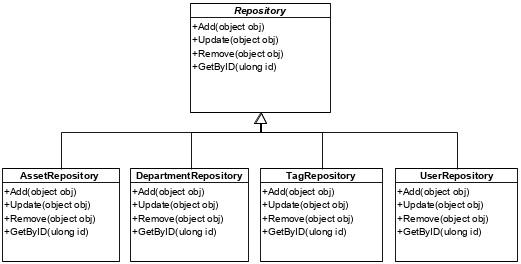
\includegraphics[width=0.8\textwidth]{figures/FunctionComponent/Repository_pattern.png}
    \caption{The repository pattern for maintaining data in the model}
    \label{fig:RepositoryPattern}
\end{figure}

\subsubsection{Attach/detach tag}
The operations of attaching or detaching an asset is called by an admin employee and involves the \textit{Tag} and \textit{Asset} classes. The functions create or delete an instance of the \textit{Asset-tag relation} class containing the involved asset and tag. The operations should be added to a class in the function component, as the admin employee does not carry out the operations. They have been placed in the \textit{AssetRepository} class, as it handles the assets. Placing them directly on the \textit{Asset} class however, would give the class responsibility of an operation in which it participate solely as an object. For clarity, the operations have been named \textit{AttachTag} and \textit{DetachTag}. Both operations take two parameters, an asset, and a list of tags to be attached to the asset.
\begin{figure}[H]
    \centering
    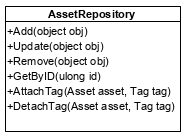
\includegraphics[width=0.3\textwidth]{figures/FunctionComponent/AttachTag.png}
    \caption{The \textit{AssetRepository} class with the \textit{AttachTag} and \textit{DetachTag} operations}
    \label{fig:AttachDetachTag}
\end{figure}

\subsubsection{Search for asset or tag}
\todo[inline]{Kommer vi til at kunne søge i comments og users skal dette også beskrives}
The 'search for asset' function lets the employee search through the assets in the system and returns the assets that comply with the search query. Multiple assets are handled and therefore it would not be intuitive to add it as an operation on the asset class. It is called by the employee, but the employee is not responsible for searching through the assets, so the function has been placed as an operation in the function component.
\par
The function 'search for tag' goes through the same process and both functions have the same structure. The search is carried out on the elements in the database and therefore they fit well into the concrete strategies of the \textit{Repository} strategy.
\begin{figure}[H]
    \centering
    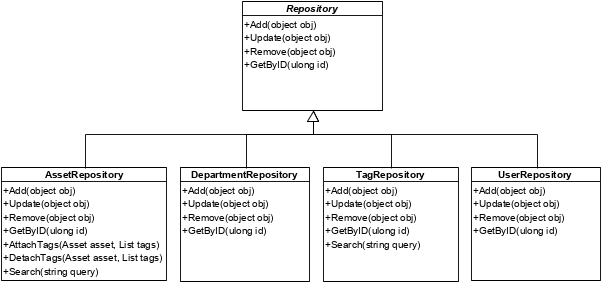
\includegraphics[width=0.8\textwidth]{figures/FunctionComponent/Repository_pattern_with_search.png}
    \caption{The repository pattern with the search operations for assets and tags}
    \label{fig:RepositoryPatternWithSearch}
\end{figure}

\subsubsection{Comment asset}
Commenting an asset adds a comment to the asset. It is desired that the comments can be retrieved and shown without knowledge about the asset to which it belongs. The reason for this is that the newest comments are to be shown on the home page of all admins, to give an overview of the latest changes and problems. Therefore the comments will not be placed directly on the asset, but will be stored separately and contain a connection to the asset. Because of this, the comment will need the functions \textit{add}, \textit{remove}, \textit{update}, and \textit{get by id} and can therefore be seen as another concrete strategy of the \textit{Repository}.
\begin{figure}[H]
    \centering
    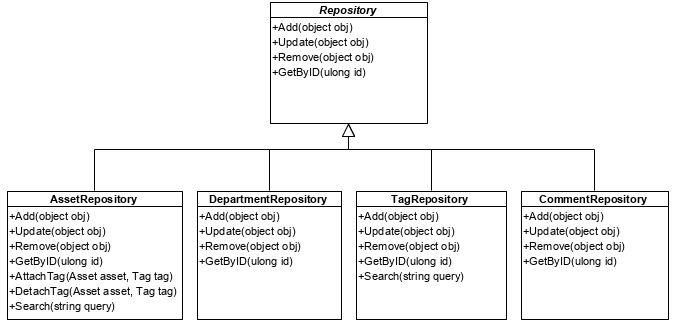
\includegraphics[width=0.9\textwidth]{figures/FunctionComponent/CommentRepository.png}
    \caption{The repository pattern with the \textit{CommentRepository}}
    \label{fig:RepositoryPatternWithCommentRepository}
\end{figure}

% \subsubsection{View asset}
% Viewing an asset means being send to a page with the asset illustrated with relevant information. The function retrieves the given asset from the database. As the function is simply reading form the database, it fits well into the \textit{MaintainModelAssets} class in the function component.
% \todo[inline]{Insert structure diagram with the new operations for asset}

\subsubsection{Authenticate user \& Check access level}
The authentication and access level check are both functions that have been handled by the \textit{Employee} class. As the employee should not do these things itself, the functions have been moved to the function component and implemented as operations in a class called \textit{Session}. They have been renamed to \textit{Authenticated} and \textit{IsAdmin} and return whether the employee currently logged into the system is authenticated and has admin authority respectively. This makes both the \textit{Employee} and \textit{Admin} classes obsolete. This class also contains the attributes \textit{Username} and \textit{Domain}, to make sure that this information about the employee currently logged in is available to the system.
\begin{figure}[H]
    \centering
    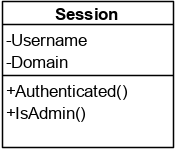
\includegraphics[width=0.3\textwidth]{figures/FunctionComponent/Session.png}
    \caption{The \textit{Session} class}
    \label{fig:session_class}
\end{figure}

\subsubsection{Export report}
The only class needing access to this function is the \textit{Admin} class. The function is not relevant to any other class, but the responsibility for executing the operation does not lie with the \textit{Admin} class itself. Therefore, the operation has been moved into a class in the function component named \textit{ExportHandler}.
\begin{figure}[H]
    \centering
    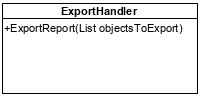
\includegraphics[width=0.4\textwidth]{figures/FunctionComponent/ExportHandler.png}
    \caption{The \textit{ExportHandler} class}
    \label{fig:ExportHandler}
\end{figure}

\subsubsection{Updating data classes}
To ensure that the data in the data classes is handled correctly, controllers have been introduced between the data classes and the related classes in the function component. This ensures that the data is correctly handled and valid, before saving it to the data classes.
\par
The controllers handle communication with classes that need information from the data classes, need to change some of the information, and also handles communication with the repositories. This makes it possible to call methods in a controller, which then formats the data class and calls the repository to maintain the database based on the changes made to the data class.
\par
The controllers differ in functionality and therefore does not build on a generalized controller. Two controllers have been depicted in the picture below (see \autoref{fig:AssetControllerAndAssetListControllerClasses}).

\begin{figure}[H]
    \centering
    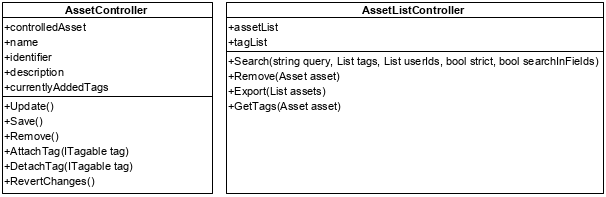
\includegraphics[width=0.9\textwidth]{figures/FunctionComponent/AssetControllerAndAssetListController.png}
    \caption{The \textit{AssetController} and \textit{AssetListController} classes}
    \label{fig:AssetControllerAndAssetListControllerClasses}
\end{figure}

The \textit{AssetController} handles only one asset and gives the surrounding classes access to the operation they need, in context of reading and updating the asset. One of these is the \textit{Save} operation, which simply calls the \textit{AssetRepository} with the controlled asset. This way, the surrounding classes do not need any knowledge of the repository to call to save the asset.
\par
The \textit{AssetListController} contains a list of assets and makes it possible for the surrounding classes to interact with the list of assets. Things such as searching through the list and removing an asset from the list. As mentioned above, the controller makes it possible for the surrounding classes to ignore the existence of certain classes, such as the repositories.

\subsubsection{Add field to asset/tag}
Adding a field to either an asset or a tag will create a field directly on the asset or tag. The fields do not have their separate place in the system, as they are not relevant without either the asset or the tag, to which they belong. Therefore the function has been implemented in the function component as an operation in an abstract class called \textit{FieldController}.
\par
The interface defines operations for adding a field to a data class, removing a field from a data class, removing a relation from a tag to every related field in the implementing controllers field list, and serializing the implementing controllers list of fields (see \autoref{fig:FieldListController}).
\par
The \textit{AddField} operation takes in two parameters. The first is the \textit{Field} that should be attached to it. The second is the object to which the field should be attached, written as the type \textit{FieldContainer}, as it can be either an asset or a tag. 
\par
The \textit{RemoveField} operation takes in the field that should be removed from the \textit{FieldContainer} class that the implementing controller is currently handling. The operation simply removes the field from the handled \textit{FieldContainer} class' list of fields.
\par
The \textit{RemoveTagRelationsOnFields} operation takes in the ID of a tag and removes all relations to fields in the implementing controllers currently handled \textit{FieldContainer} class field list.\\
The last method is used to serialize the field in the implementing controllers currently handled \textit{FieldContainer} class field list.

\begin{figure}[H]
    \centering
    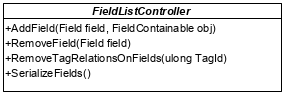
\includegraphics[width=0.5\textwidth]{figures/FunctionComponent/FieldListController.png}
    \caption{The \textit{FieldListController} class}
    \label{fig:FieldListController}
\end{figure}

\subsubsection{ViewModels}

\subsection{Specification of complex functions}
The complex functions have been depicted with further descriptions, to ease the understanding of the process of them. Some of the complex function are trivial and therefore have not been described in further detail. This includes the search assets and tags operations.
% This includes the adding and removing of assets, departments, and tags, updating these as it is simply changing the value of attributes, and searching through the sets.
\par
This leaves the Export report function to be described in further detail.
\begin{table}[H]
    \centering
    \hrule
    \begin{tabular}{p{5cm} p{8cm}}
    \\
         \textbf{Name} & Export report \\\\
         \textbf{Category} & Passive read\\\\
         \textbf{Purpose} & Creates a CSV-file and saves it on the users computer.\\\\
         \textbf{Input data} & Collection of elements to be exported in the CSV-file.\\\\
         \parboxc{t}{1ex}{\textbf{Conditions}} & The user has selected one or more elements to be exported.\newline A location on the users computer to store the file.\\\\
         \textbf{Effect} & A CSV-file containing the collection of elements is created.\\\\
         \textbf{Algorithm} & -\\\\
         \textbf{Data structures} & Enumerable list\\\\
         \textbf{Placement} & ExportHandler\\\\
         \textbf{Involved objects} & Asset\\\\
         \textbf{Triggering events} & export report\\\\
    \end{tabular}
    \hrule
    \caption{Specification of the \textit{Export report} operation}
    \label{tab:complex_func_description_export_report}
\end{table}
\par
The overall behaviour of the system is pretty simple, as it only has the state \textit{active}. Therefore, a diagram of this behaviour is trivial and has not been included here.
\par
The function component has then been constructed and is illustrated below in \autoref{fig:FunctionComponent}.
\begin{figure}[H]
    \centering
    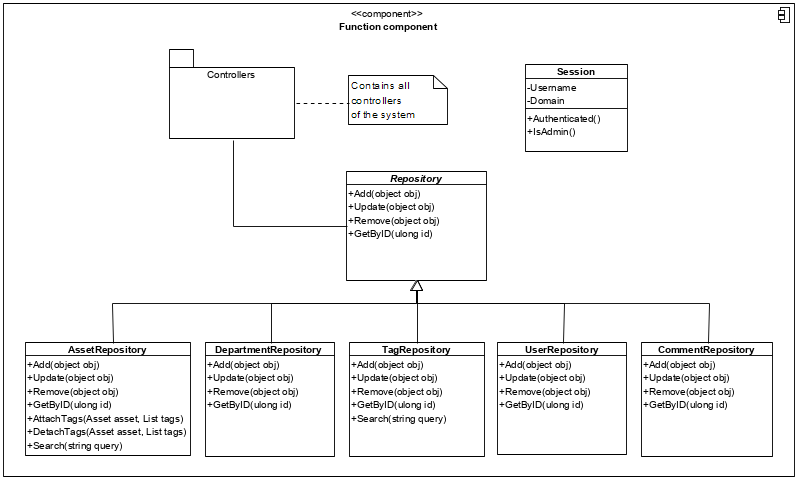
\includegraphics[width=0.8\textwidth]{figures/FunctionComponent/FunctionComponent.png}
    \caption{Illustration of the function component of the system}
    \label{fig:FunctionComponent}
\end{figure}